\documentclass[a4paper]{article}
\usepackage[margin = 1 in]{geometry}
\usepackage{fancyhdr}
\usepackage{lastpage}
\usepackage{ctex}
\usepackage[utf8]{inputenc} % Required for inputting international characters
\usepackage[T1]{fontenc} % Output font encoding for international characters
\usepackage[sfdefault]{ClearSans} % Use the Clear Sans font (sans serif)
\usepackage{tocloft} 
\usepackage[hidelinks]{hyperref}
\usepackage{makecell}%导入表格宏包
\usepackage{bmpsize}
\usepackage{graphicx}
\usepackage{epstopdf}
\usepackage{caption}
\usepackage{enumitem}
\usepackage{float}
\usepackage{multirow}
\usepackage{makecell}

\pagestyle{fancy}
\lhead{\textsl{Final Year Project}}
\chead{}
\rhead{Page \thepage\ of \pageref{LastPage}}
\lfoot{}
\rfoot{}
\cfoot{}
\renewcommand{\headrulewidth}{0.4pt}
\renewcommand{\footrulewidth}{0pt}
\renewcommand{\cftsecleader}{\cftdotfill{\cftdotsep}}
\newcommand{\tabincell}[2]{\begin{tabular}{@{}#1@{}}#2\end{tabular}} %单元格内换行

\renewcommand*\contentsname{Table of Contents}

\begin{document}

%----------------------------------------------------------------------------------------
%	TITLE PAGE
%----------------------------------------------------------------------------------------

\begin{titlepage}
	
	\rule{\linewidth}{5pt}
	\raggedleft
	\fontsize{38pt}{50pt}\selectfont
    \textbf{\\Team Project\\}
    \fontsize{28pt}{60pt}\selectfont 
    for\\
    \fontsize{38pt}{60pt}\selectfont 
    \textbf{Milestone 1\\}
	
	\vfill % Space between the title box and author information
	
	%------------------------------------------------
	%	Author name and information
	%------------------------------------------------
	
	\parbox[t]{0.93\textwidth}{ % Box to inset this section slightly
		\raggedleft % Right align the text
		\large % Increase the font size
		{\Large By Zijun Li\_2272583\_zxl183}\\[4pt] % Extra space after name
	}
	
\end{titlepage}

\begin{center}
	\tableofcontents
	\addcontentsline{toc}{section}{Table of Contents}
\end{center}
\newpage

\section{Agreed, coherent project concept \& personas \& mockups}

\subsection{Project concept}

In the digital age, where information overload is a common issue, the ability to skim through news without missing essential content becomes crucial. "Mirror News Summarizer" serves this need by offering users a streamlined version of their favorite news portals with the added advantage of concise summaries, allowing for efficient consumption of news. Recognizing the diverse interests of readers and the importance of personalization, we aim to take this platform a step further by integrating a sophisticated recommendation page. This unique feature stands to revolutionize the user experience by curating news articles based on popularity and user interaction within the mirrored sites, all housed within a separate, dedicated page.

\begin{enumerate}[wide, labelwidth=!, labelindent=0pt, label=\textbf{\arabic*.}]
    \item \textbf{Quick News Overview}: 
    Users can swiftly get the gist of articles through intelligent summarization, allowing them to consume more information in less time. Each piece retains key points and facts, ensuring a comprehensive understanding without the need for full-length reading.

    \item \textbf{Familiar Interface Design}: 
    The mirror aspect maintains the original website design, providing a comfortable and familiar browsing experience. Users navigate as usual, but with the benefit of quick, summarized content.

    \item \textbf{Personalized Recommendations}: 
    A dedicated page offers users a list of articles resonating with a wider audience, powered by real-time analysis of clicks and reads across the platform. It’s not just what’s trending globally; it’s what like-minded individuals are reading.

    \item \textbf{Interest-Based Curation}:
    Over time, the system learns from individual user interactions, allowing for a more tailored article suggestion list that aligns with their reading preferences and interests.

    \item \textbf{Engagement Through Feedback}:
    Users have the opportunity to react to summaries and recommended articles, providing feedback that enhances and personalizes their news consumption journey. This input directly influences future summarization and recommendation quality.
\end{enumerate}

\subsection{mockups}

\subsubsection{Main Page}

\begin{figure}[H] %H为当前位置,!htb为忽略美学标准,htbp为浮动图形
	\centering %图片居中
	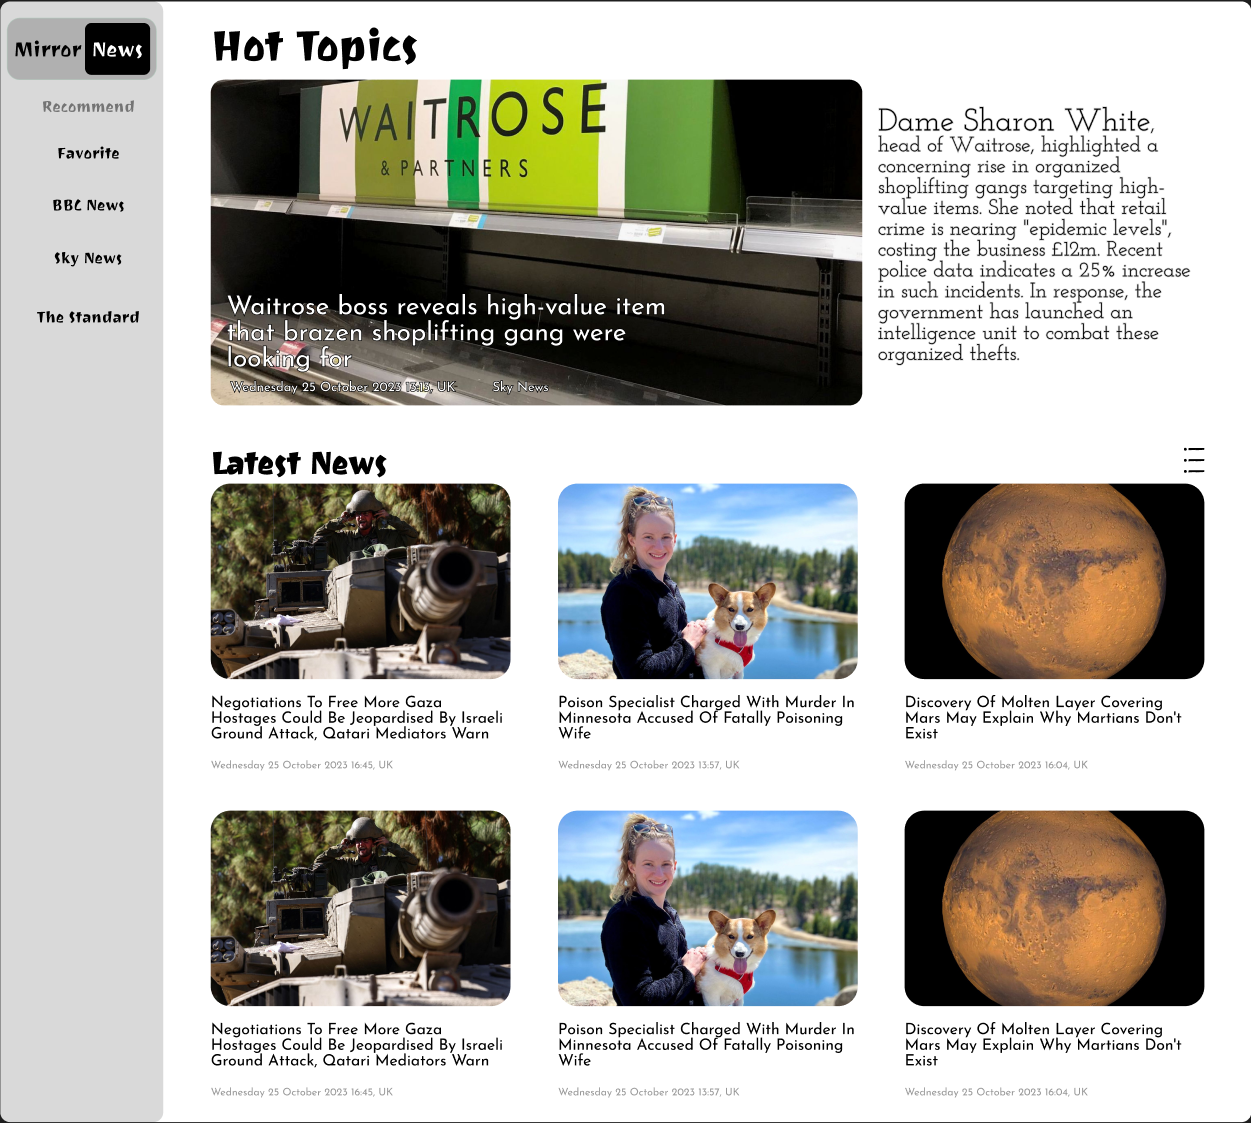
\includegraphics[width=0.8\textwidth]{./images/Main Page.png} %插入图片,[]中设置图片大小,{}中是图片文件名
	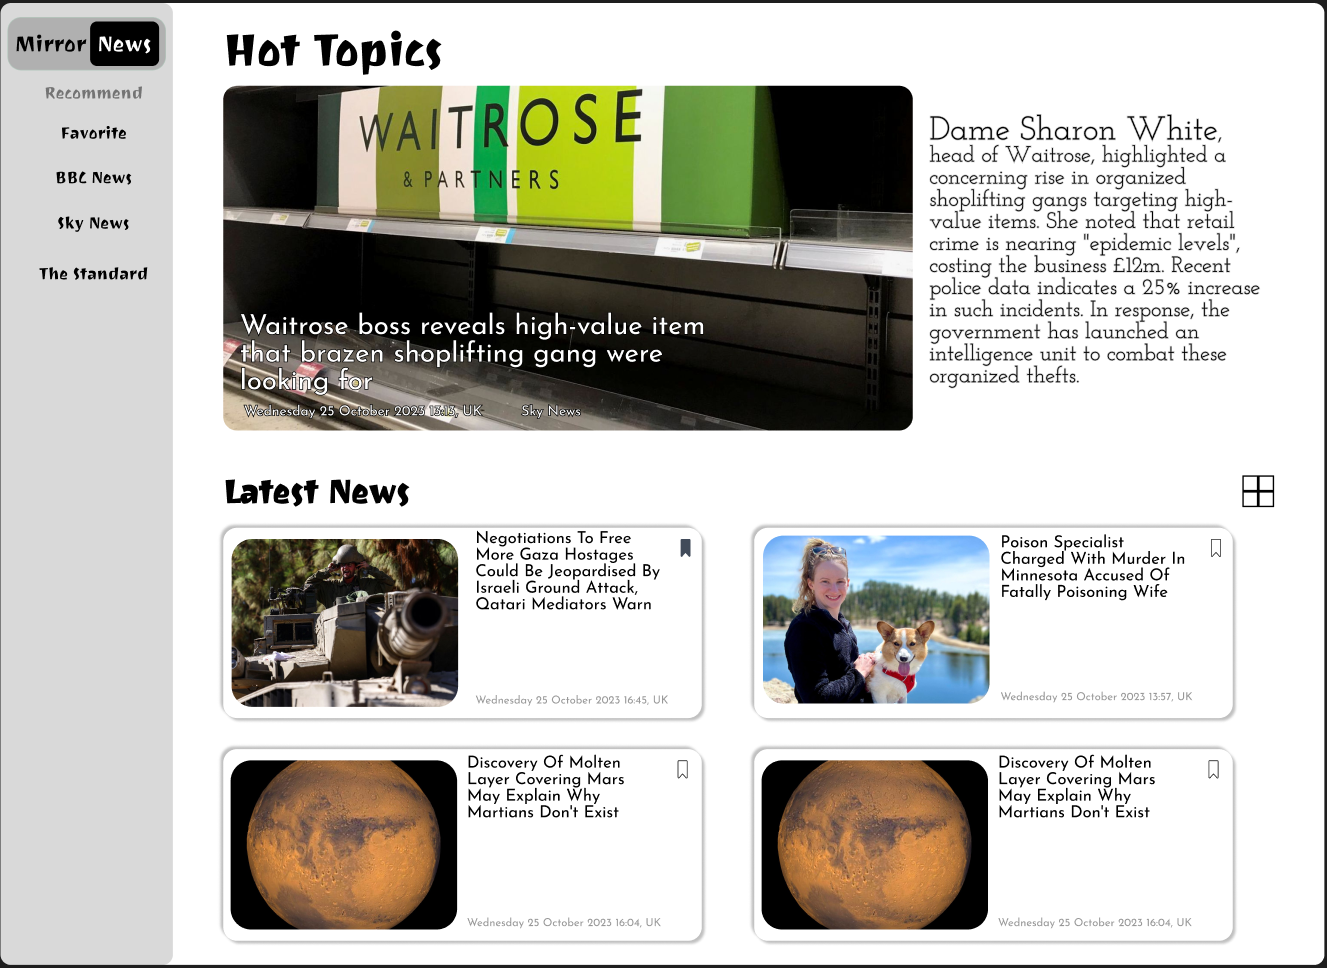
\includegraphics[width=0.8\textwidth]{./images/Main Page 2.png} %插入图片,[]中设置图片大小,{}中是图片文件名
	\caption*{Main Page} %最终文档中希望显示的图片标题
	\label{Fig.Main Page} %用于文内引用的标签
\end{figure}

\subsubsection{Recommend}

\begin{figure}[H] %H为当前位置,!htb为忽略美学标准,htbp为浮动图形
	\centering %图片居中
	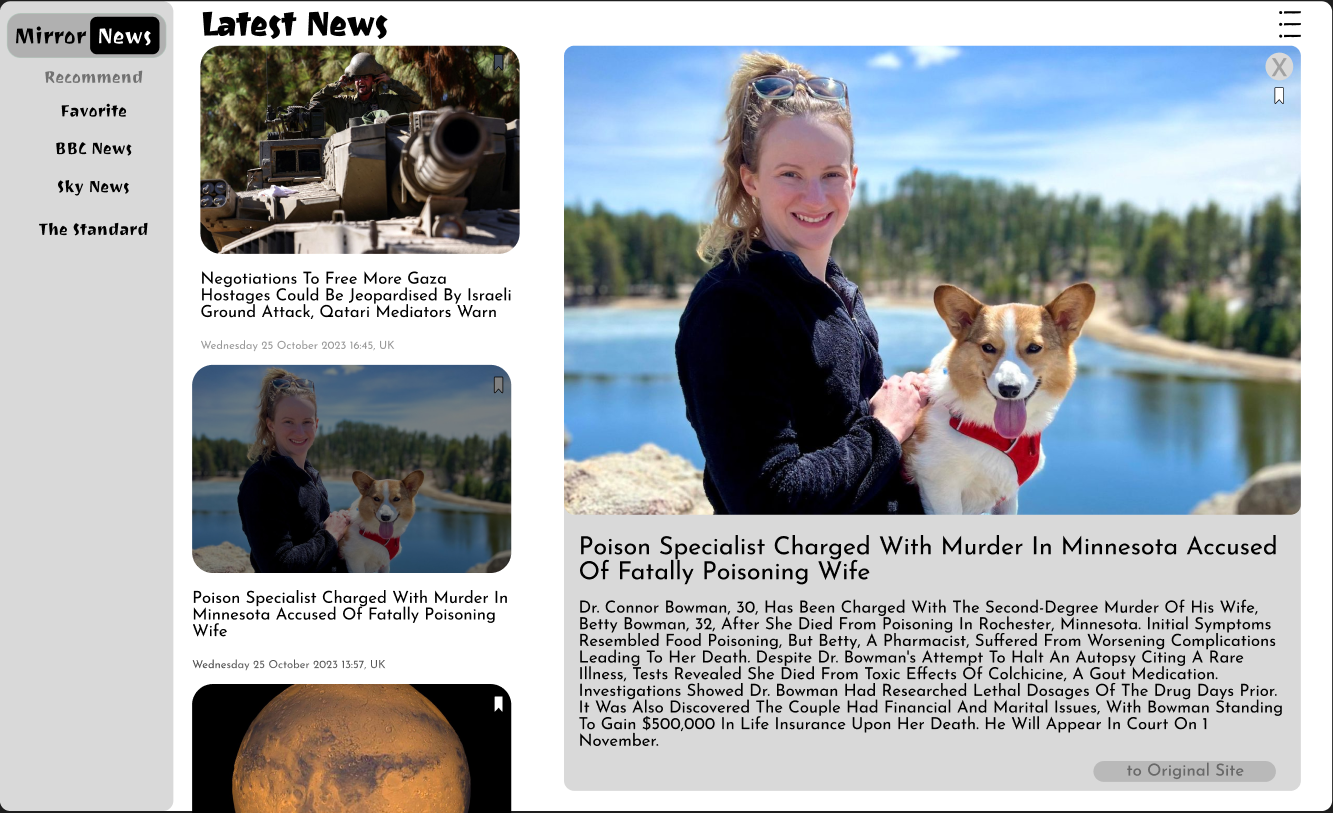
\includegraphics[width=1\textwidth]{./images/Recommand.png} %插入图片,[]中设置图片大小,{}中是图片文件名
	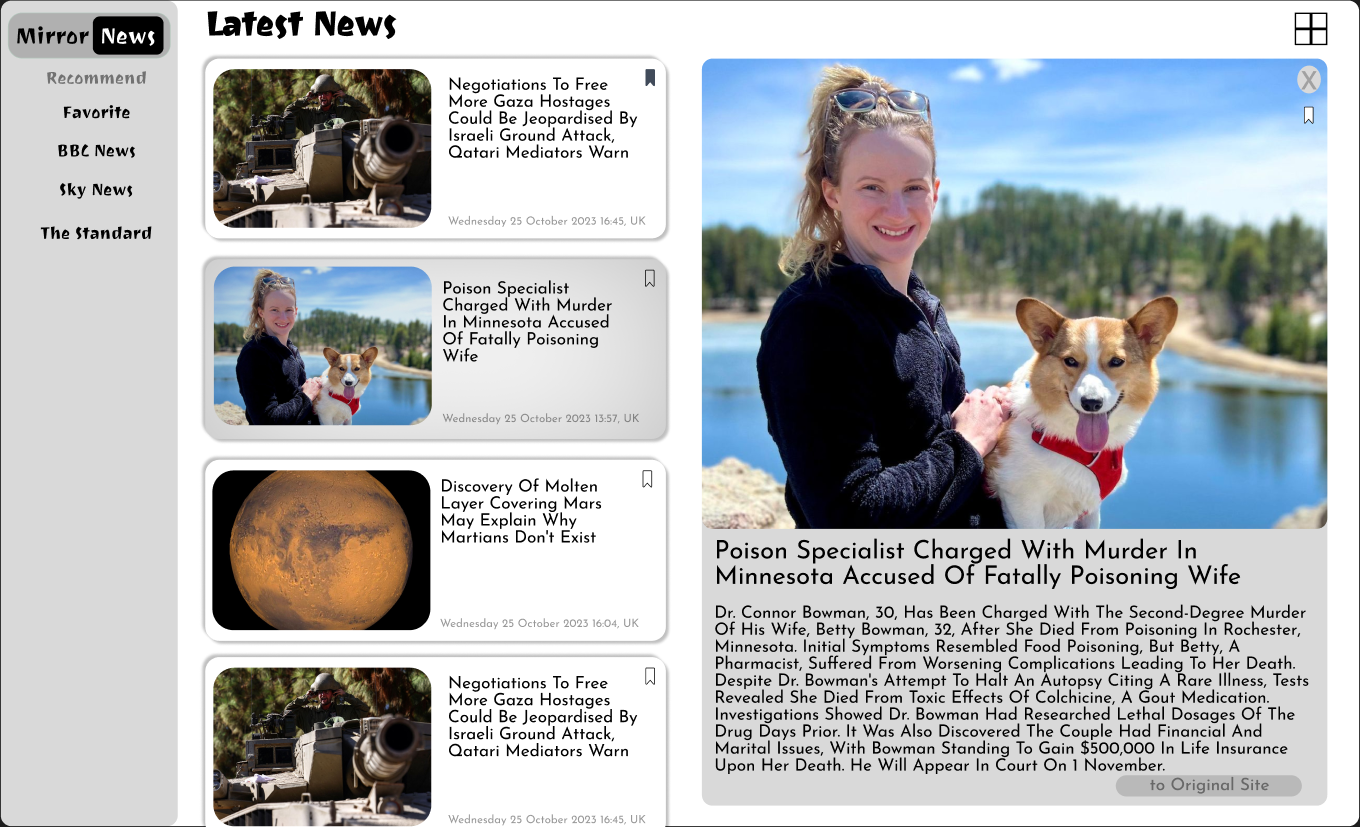
\includegraphics[width=1\textwidth]{./images/Recommand 2.png} %插入图片,[]中设置图片大小,{}中是图片文件名
	\caption*{Recommand} %最终文档中希望显示的图片标题
	\label{Fig.Recommand} %用于文内引用的标签
\end{figure}

\subsubsection{Favorite}

\begin{figure}[H] %H为当前位置,!htb为忽略美学标准,htbp为浮动图形
	\centering %图片居中
	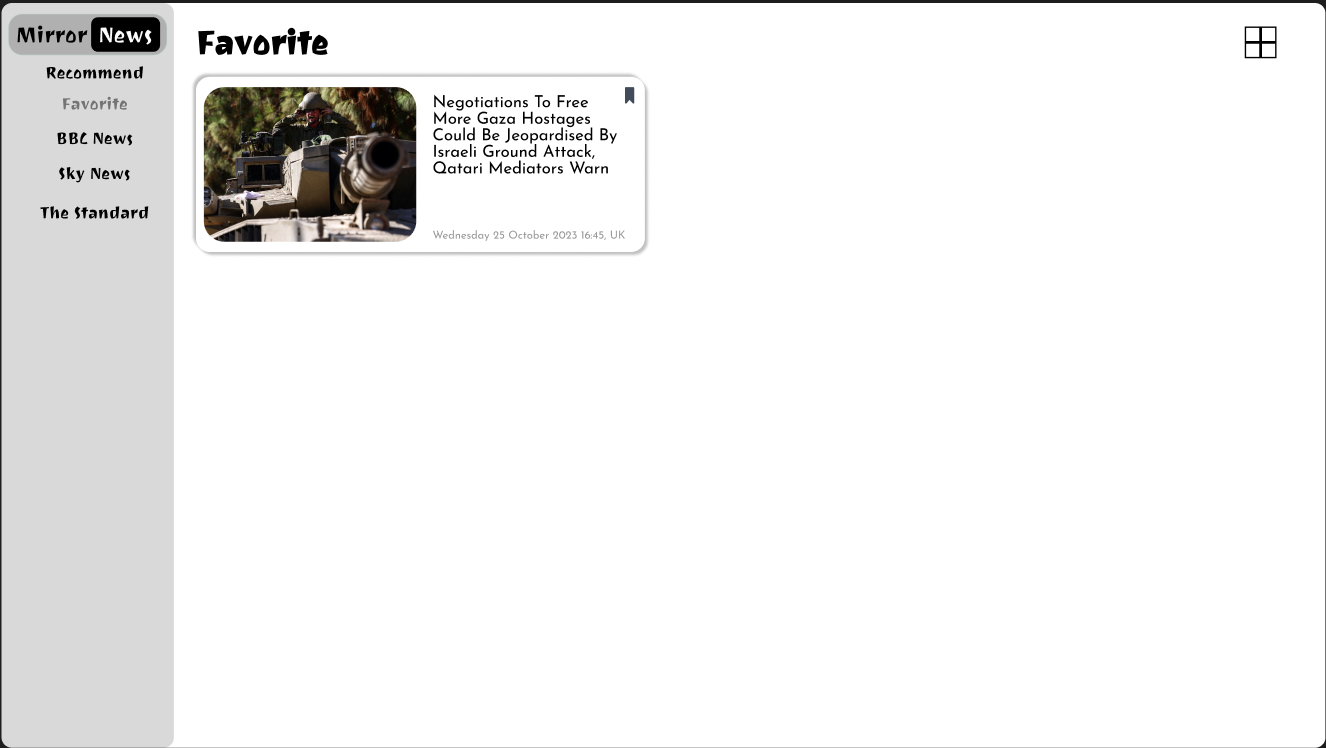
\includegraphics[width=1\textwidth]{./images/Favorite.png} %插入图片,[]中设置图片大小,{}中是图片文件名
	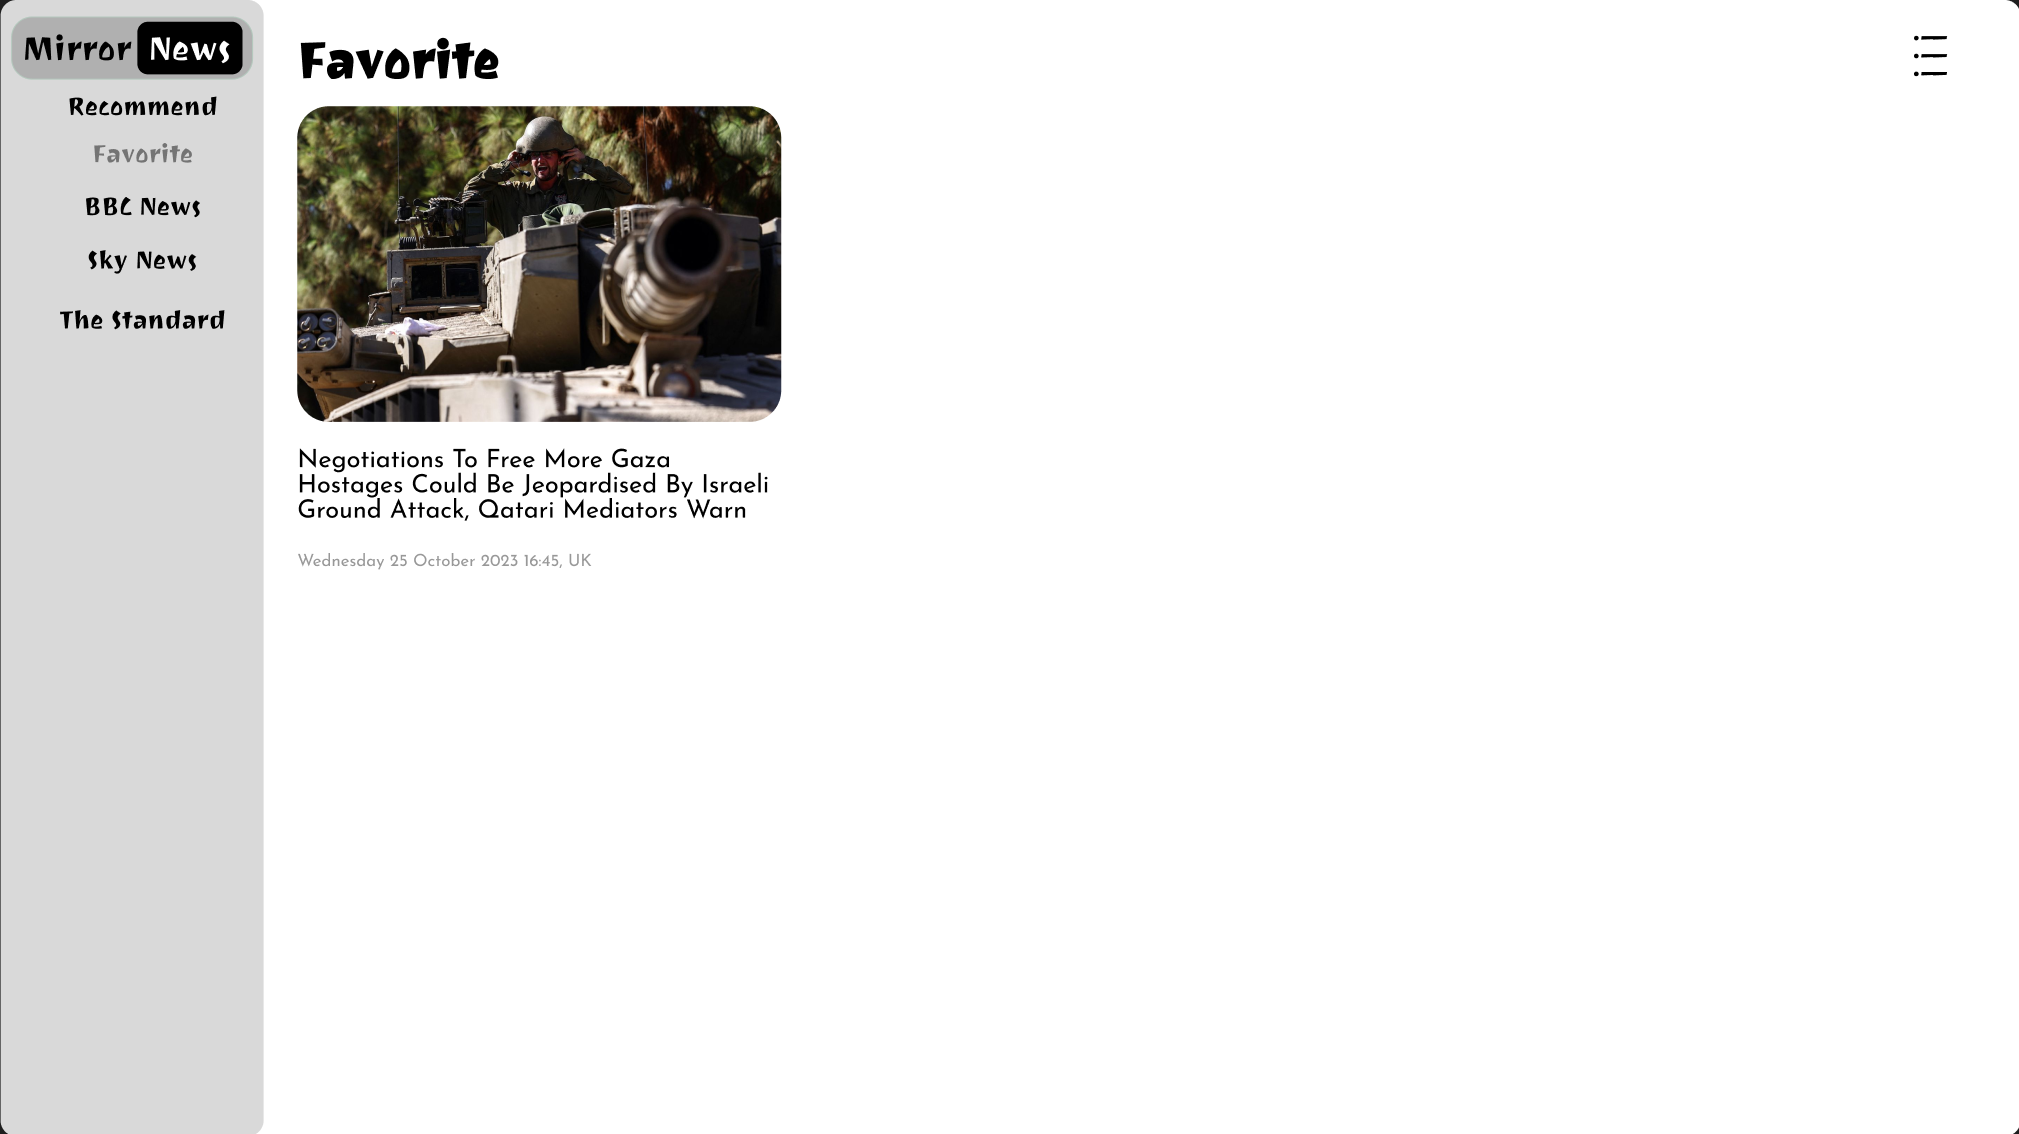
\includegraphics[width=1\textwidth]{./images/Favorite 2.png} %插入图片,[]中设置图片大小,{}中是图片文件名
	\caption*{Favorite} %最终文档中希望显示的图片标题
	\label{Fig.Favorite} %用于文内引用的标签
\end{figure}

\subsubsection{Sky News}

\begin{figure}[H] %H为当前位置,!htb为忽略美学标准,htbp为浮动图形
	\centering %图片居中
	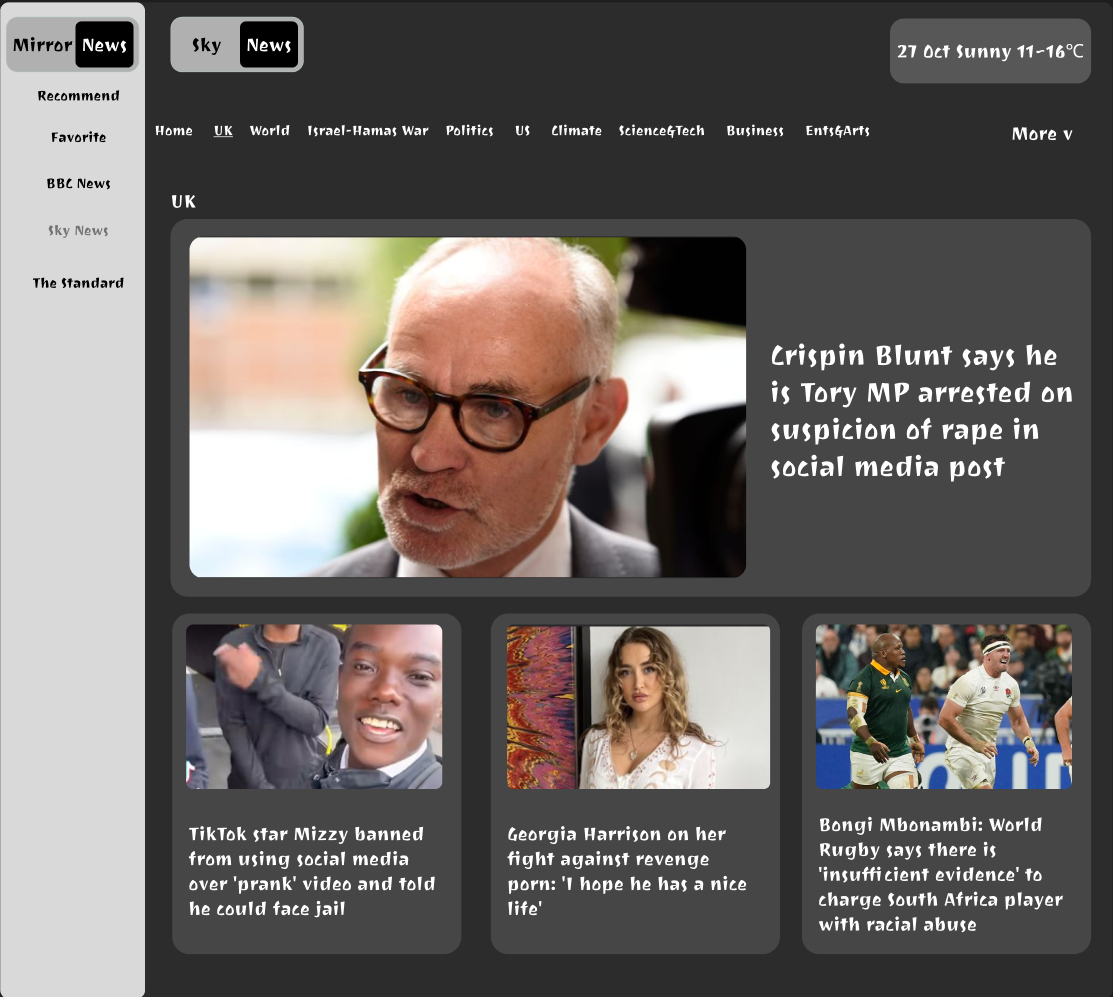
\includegraphics[width=0.7\textwidth]{./images/Sky news 2.png} %插入图片,[]中设置图片大小,{}中是图片文件名
	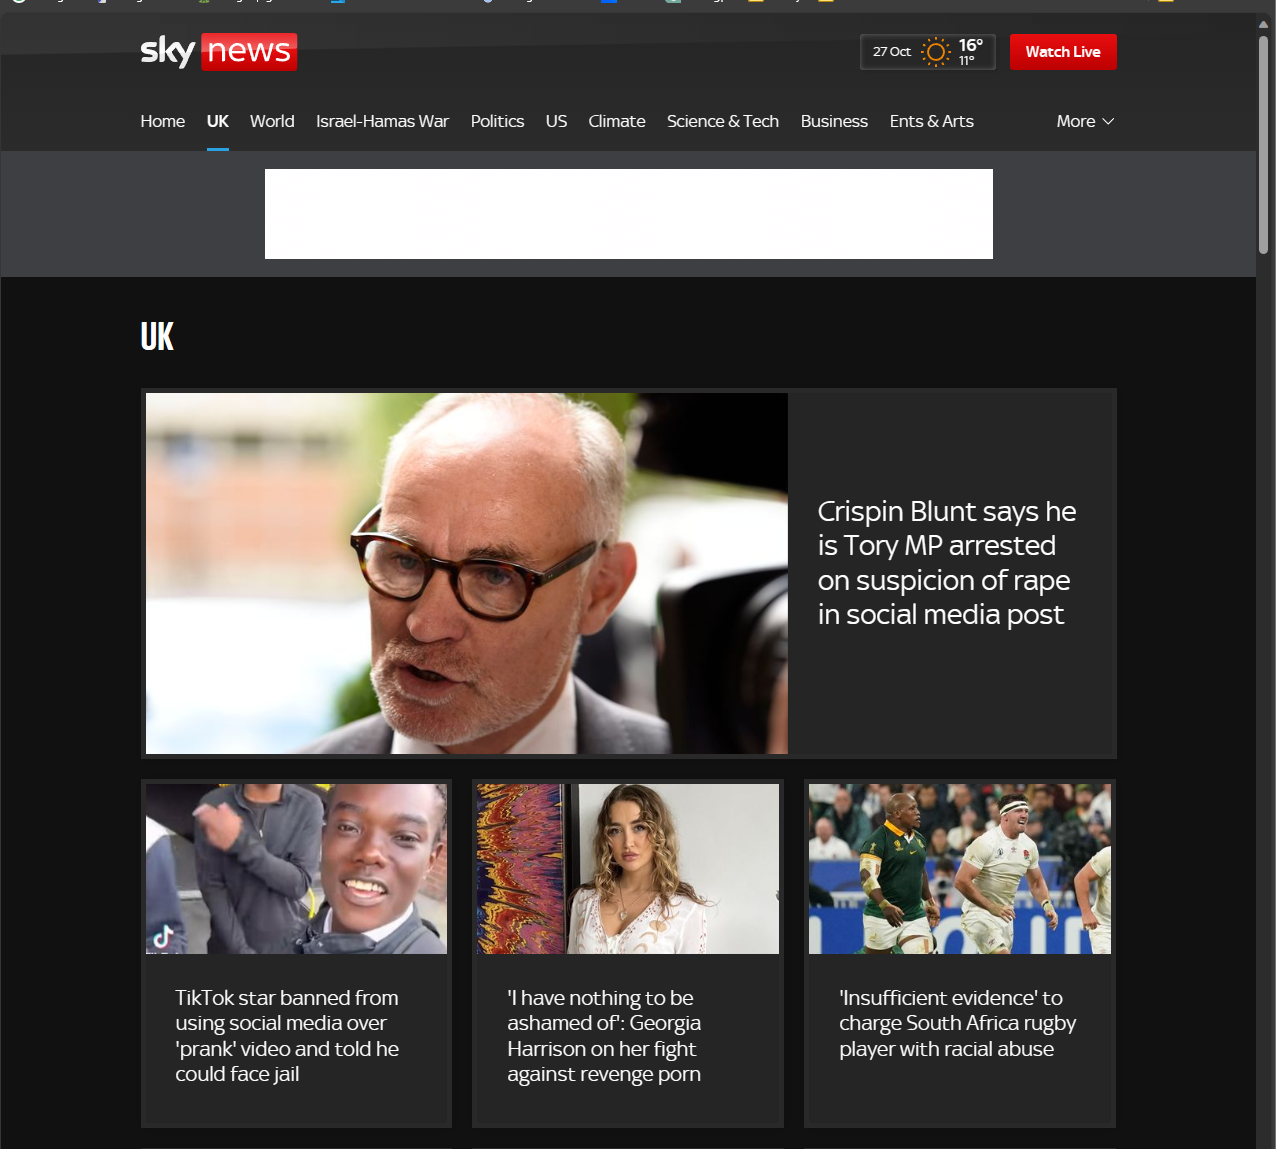
\includegraphics[width=0.7\textwidth]{./images/Sky news.png} %插入图片,[]中设置图片大小,{}中是图片文件名
	\caption*{Sky News} %最终文档中希望显示的图片标题
	\label{Fig.Sky News} %用于文内引用的标签
\end{figure}

\subsection{Persona}

\begin{figure}[H] %H为当前位置,!htb为忽略美学标准,htbp为浮动图形
	\centering %图片居中
	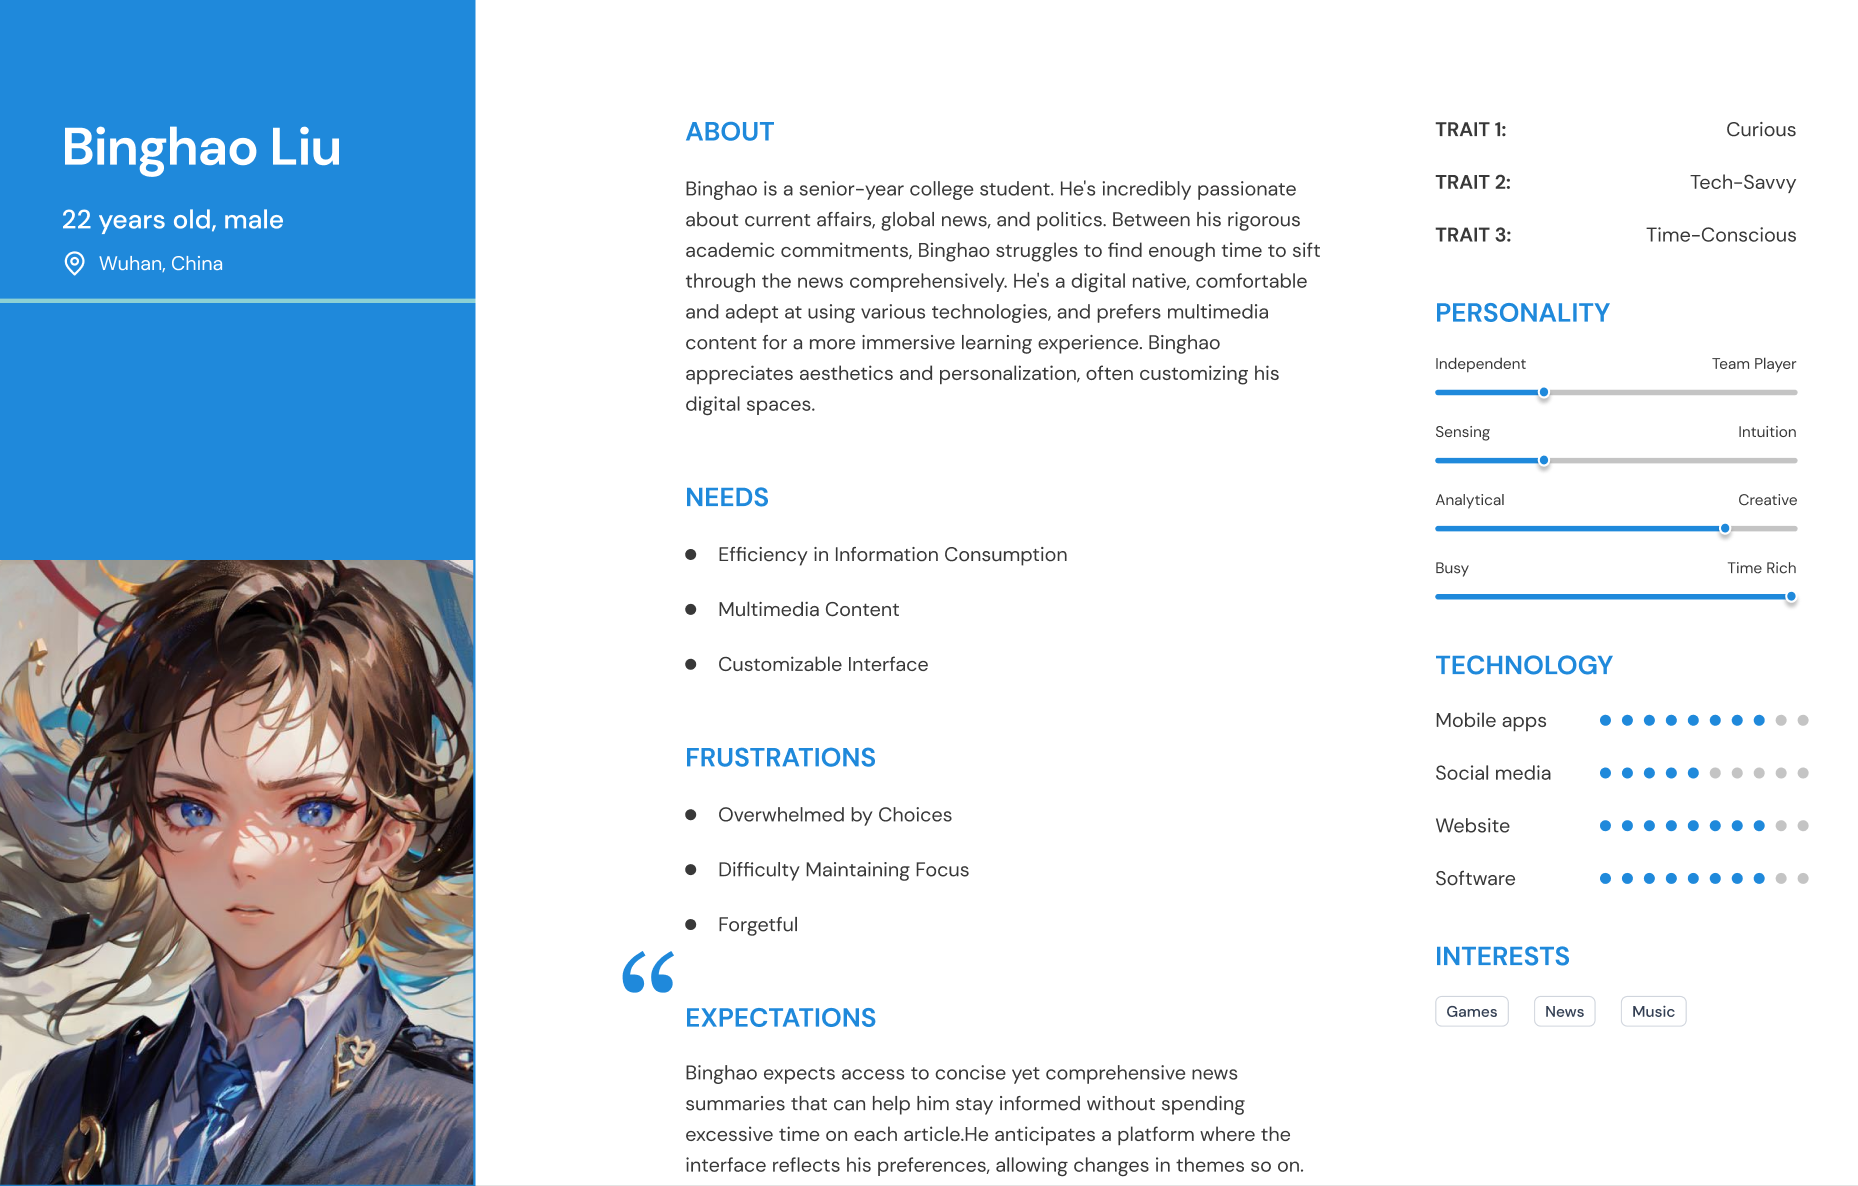
\includegraphics[width=1\textwidth]{./images/Persona_1.png} %插入图片,[]中设置图片大小,{}中是图片文件名
	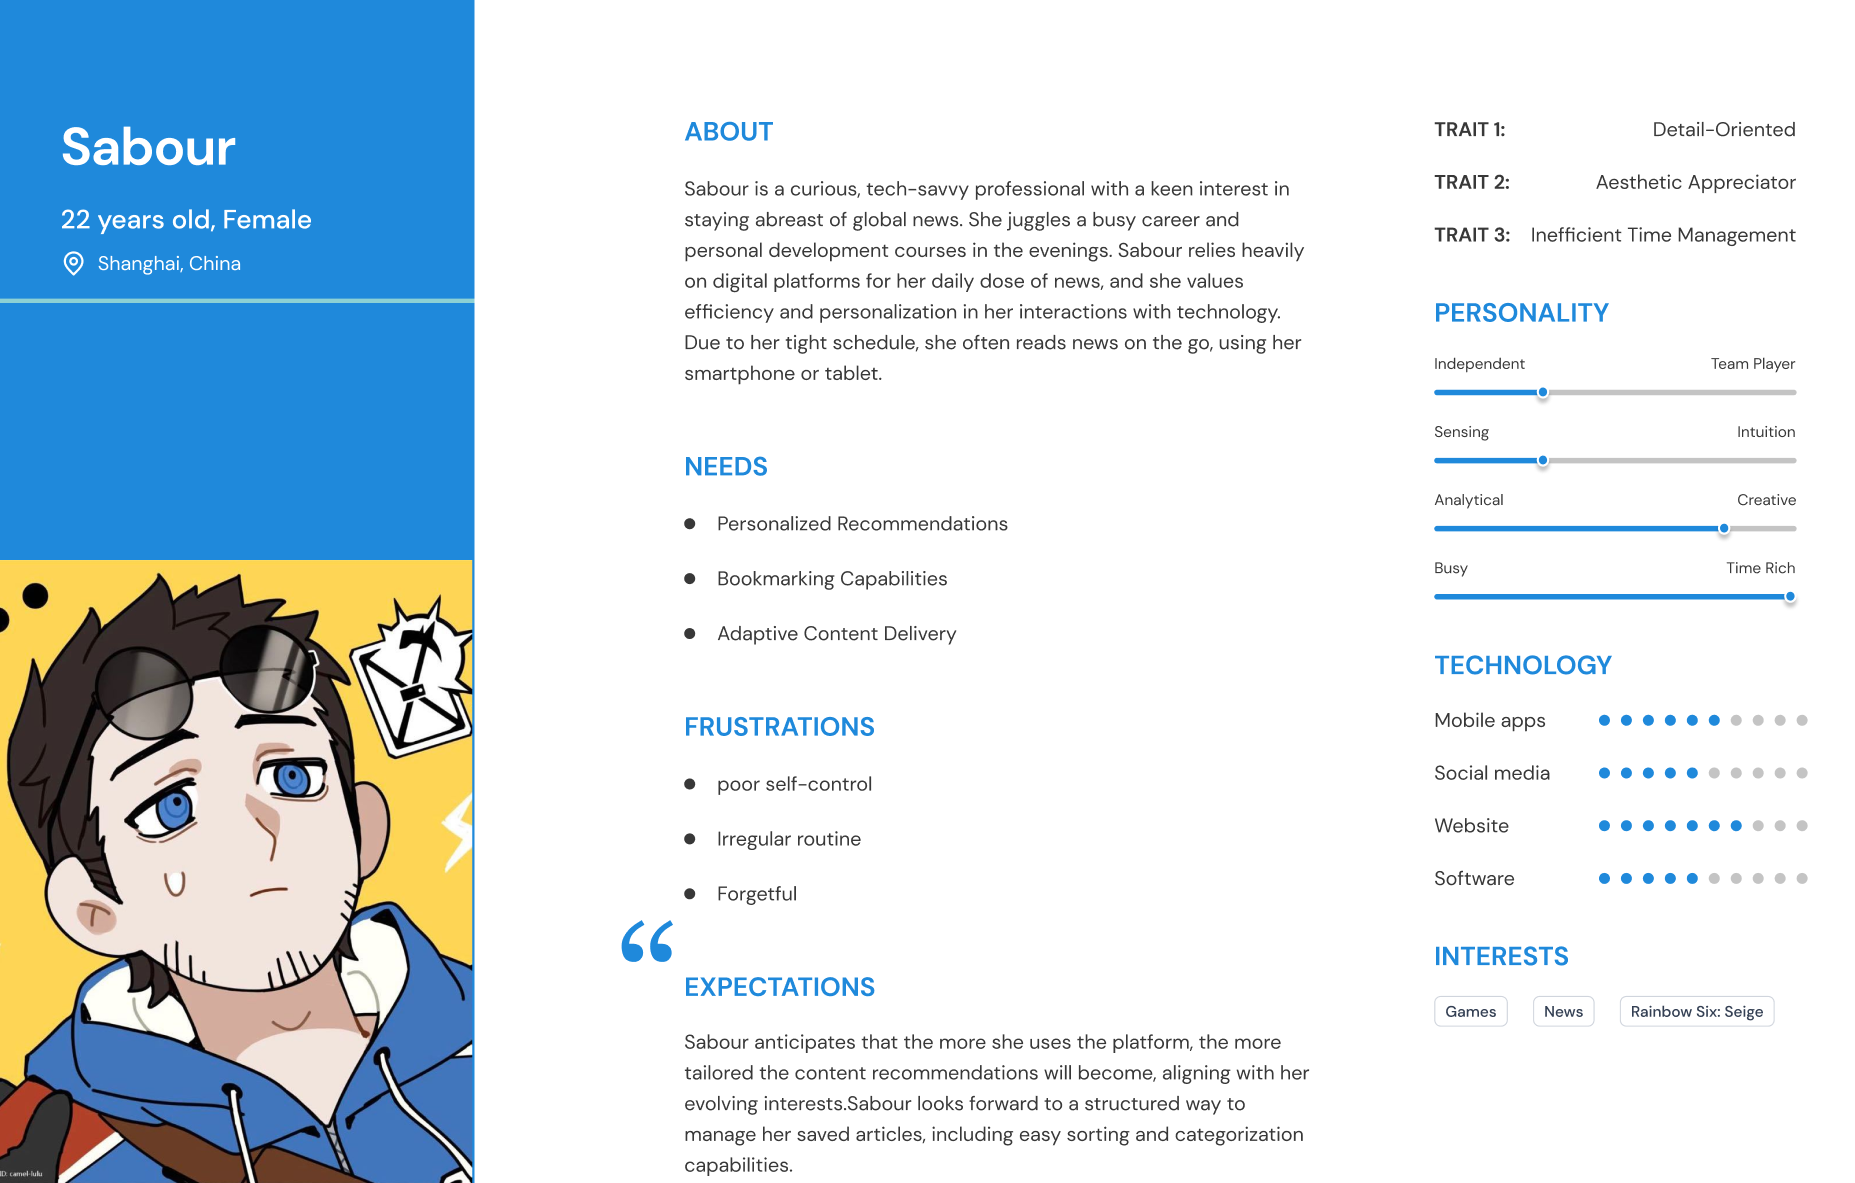
\includegraphics[width=1\textwidth]{./images/Persona_2.png}
	\caption*{} %最终文档中希望显示的图片标题
	\label{Fig.Personas1} %用于文内引用的标签
\end{figure}

\newpage

\begin{figure}[H] %H为当前位置,!htb为忽略美学标准,htbp为浮动图形
	\centering %图片居中
	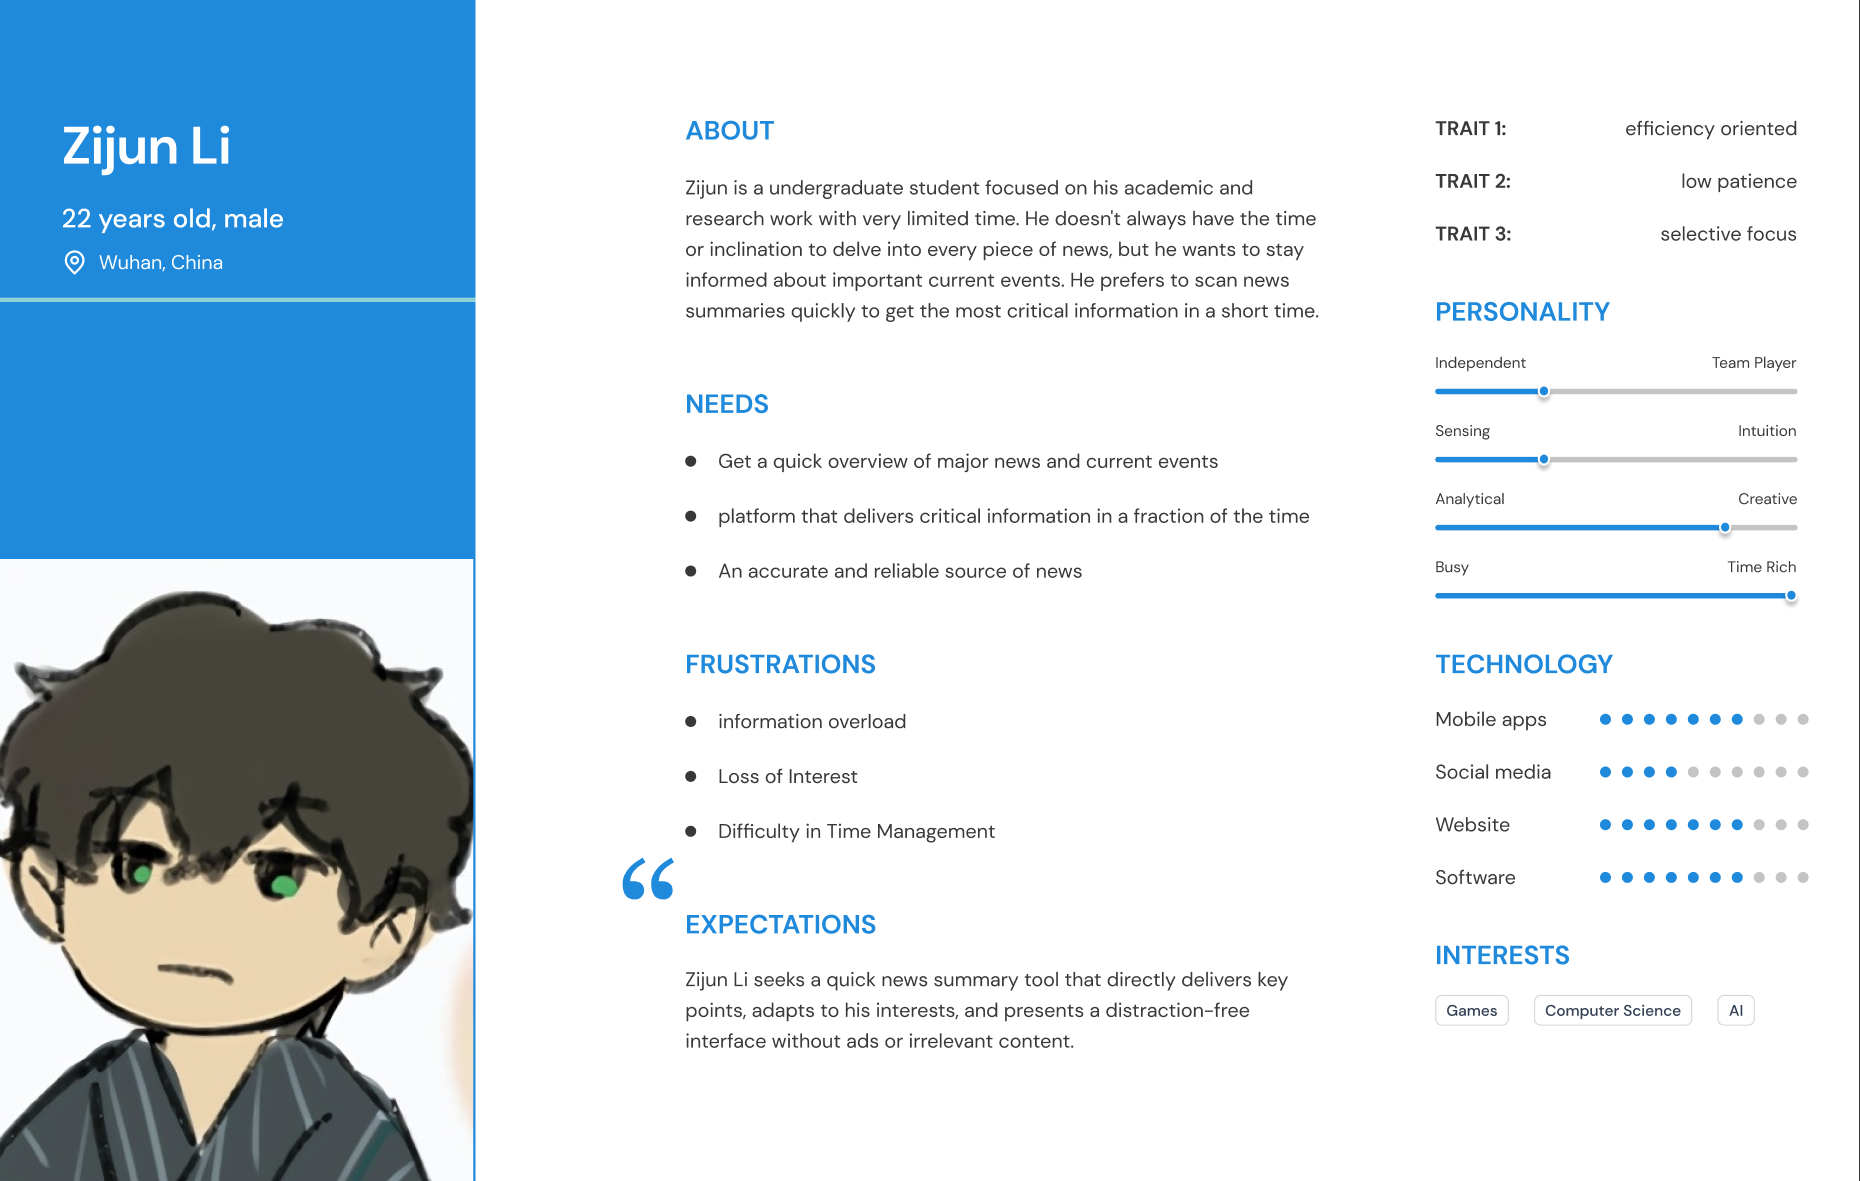
\includegraphics[width=1\textwidth]{./images/Persona_3.png} %插入图片,[]中设置图片大小,{}中是图片文件名
	\caption*{} %最终文档中希望显示的图片标题
	\label{Fig.Persona2} %用于文内引用的标签
\end{figure}

\end{document}